\begin{wrapfigure}{l}{0.1\textwidth}
	\vspace{-10pt}
	
\includegraphics[width=\linewidth]{images/ikony_pliki.png}
\end{wrapfigure}

Menadżer plików jest programem służącym do przeglądania zawartości katalogów. W Ubuntu menadżerem plików jest program  \textcolor{ubuntu_orange}{Pliki} (wcześniejsza, ale nadal używana nazwa, to \textcolor{ubuntu_orange}{Nautilus}), który jest odpowiednikiem programu \textcolor{ubuntu_orange}{Eksplorator Windows} z systemów Windows oraz \textcolor{ubuntu_orange}{Finder} z MacOX X. Na pasku Launchera domyślnie drugą ikoną jest ikona Nautilusa. 

Program Pliki po uruchomieniu wyświetla zawartość katalogu domowego, w którym użytkownik przechowuje swoje osobiste pliki. Każdy użytkownik ma swój oddzielny katalog domowy, którego nazwa odpowiadania nazwie użytkownika. Po utworzeniu konta w katalogu domowym automatycznie tworzone są katalogi Dokumenty, Muzyka, Obrazy, Pobrane, Publiczny, Pulpit, Szablony, Wideo. Użytkownik nie jest ograniczony jedynie do nich i bez problemu w katalogu domowym może stworzyć więcej katalogów i plików.

Menadżer plików w lewym panelu będzie też wyświetlał podłączone urządzenia (pendrive'y, karty SD, płyty włożone do napędów optycznych) oraz udziały sieciowe (inne podłączone komputery). Pozycja \textcolor{ubuntu_orange}{Komputer} przenosi do początku systemu plików (katalog /).

\begin{center}
	\begin{tikzpicture}
	\node[anchor=south west,inner sep=0] (image) at (0,0) {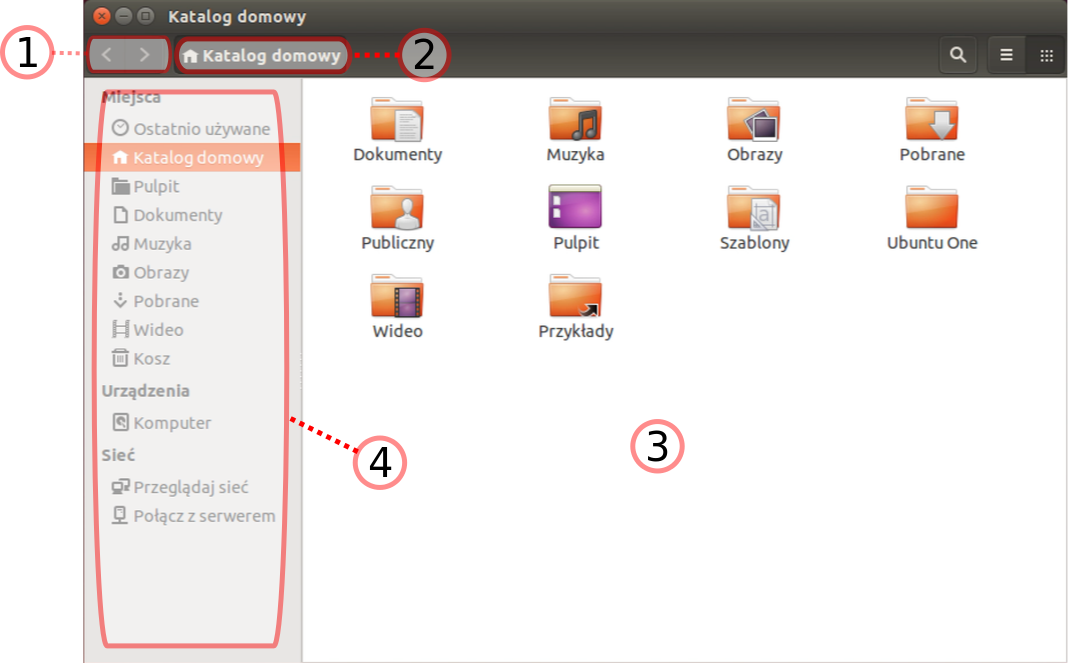
\includegraphics[width=\linewidth]{images/programy_nautilus.png}};
	\begin{scope}[x={(image.south east)},y={(image.north west)}]
		\draw[ubuntu_orange,line width=3pt,rounded corners] (0.005,0.88) rectangle (0.085,0.95);
		\draw[ubuntu_orange,line width=3pt,fill=white,fill opacity=0.75] (0.35,0.96) circle [radius=0.30cm]
			node[text=black]{\Large \textbf 1};
		\draw[ubuntu_orange,dashed,line width=3pt] (0.33,0.96) -- (0.05,0.98) -- (0.05,0.95);
		
		\draw[ubuntu_orange,line width=3pt,rounded corners] (0.085,0.88) rectangle (0.27,0.95);
		\draw[ubuntu_orange,line width=3pt,fill=white,fill opacity=0.75] (0.35,0.89) circle [radius=0.30cm]
			node[text=black]{\Large \textbf 2};
		\draw[ubuntu_orange,dashed,line width=3pt] (0.33,0.89) -- (0.27,0.89);
		
		\draw[ubuntu_orange,line width=3pt,fill=white,fill opacity=0.75] (0.55,0.35) circle [radius=0.30cm]
			node[text=black]{\Large \textbf 3};
					
		\draw[ubuntu_orange,line width=3pt,rounded corners] (0.005,0.005) rectangle (0.22,0.87);
		\draw[ubuntu_orange,line width=3pt,fill=white,fill opacity=0.75] (0.1,0.1) circle [radius=0.30cm]
			node[text=black]{\Large \textbf 4};

    \end{scope}
\end{tikzpicture}
\end{center}


W oknie menadżera plików widzimy:
\begin{enumerate}[label=\protect\circled{\arabic*}]
\item przyciski \textcolor{ubuntu_orange}{Do tyłu} i \textcolor{ubuntu_orange}{Do przodu};
\item aktualne położenie;
\item zawartośc aktualnego katalogu;
\item pasek ze skrótami do najważniejszych miejsc.
\end{enumerate}

Do nawigacji w pasku narzędzi oraz lewym panelu wykorzystywane jest pojedyncze kliknięcie lewym przyciskiem myszy. W prawym panelu pliki oraz katalogi domyślnie otwieramy dwukrotnym szybkim przyciśnięciem lewego przycisku myszy. W przypadku otwarcia pliku, Ubuntu rozpozna typ pliku i automatycznie spróbuje przypisać odpowiednią dla danego pliku aplikację. Czasami system może nie rozpoznać typu pliku lub może zajść potrzeba otwarcia pliku w innym programie. W takich wypadkach, po dwukrotnym kliknięciu pliku system zapyta, który program z zainstalowanych w systemie chcemy wykorzystać. Możemy również kliknąć plik prawym przyciskiem myszy i z menu kontekstowego wybrać ,,Otwórz za pomocą'', a następnie wybrać z listy dostępnych programów lub samemu wskazać inny.

Najważniejsze katalogi w folderze użytkownika:
\begin{itemize}
\item \textcolor{ubuntu_orange}{Pulpit} --- wszystkie pliki i foldery umieszczone w tym katalogu zostaną wyświetlone na pulpicie.
\item \textcolor{ubuntu_orange}{Dokumenty} --- katalog na dokumenty, pliki tekstowe, arkusze kalkulacyjne, itp.
\item \textcolor{ubuntu_orange}{Muzyka} --- katalog z plikami muzycznymi. Odtwarzacze muzyki będą szukać plików do odtwarzania najpierw w tym folderze.
\item \textcolor{ubuntu_orange}{Wideo} --- katalog z plikami wideo.
\item \textcolor{ubuntu_orange}{Obrazy} --- katalog z fotografiami.
\item \textcolor{ubuntu_orange}{Pobrane} --- katalog na pliki pobrane z internetu. Przeglądaki internetowe domyślnie będą zapisywać pobrane pliki w tym katalogu.
\end{itemize}

\subsubsection{Tworzenie nowych katalogów}
Tworzenie nowych katalogów przebiega identycznie, jak w innych systemach. Wystarczy po prostu kliknąć prawym przyciskiem myszy wolną przestrzeń w oknie programu (ta metoda również zadziała na pulpicie) i z menu kontekstowego wybrać opcję \textcolor{ubuntu_orange}{Nowy katalog}. Można również wykorzystać w tym celu panel menu i wybrać \menu{Plik>{Nowy katalog}}, albo wcisnąć kombinację klawiszy \keys{Shift + CTRL + n}.

\subsubsection{Ukryte pliki i katalogi}
Ubuntu, jak każdy inny linux, umożliwia tworzenie ukrytych plików i katalogów. Aby ukryć plik lub katalog, wystarczy w jego nazwie na samym początku wstawić kropkę (.). Gdy chcemy uzyskać dostęp do ukrytych plików lub katalogów, należy z panelu menu wybrać \menu{Widok>Wyświetlanie ukrytych plików} lub wcisnąć kombinację klawiszy \keys{CTRL + h}.

UWAGA: Wyświetlenie ukrytych plików w katalogu domowym użytkownika wyświetli wiele dodatkowych plików i katalogów, które w większości przypadków przechowują ustawienia wielu programów, wyglądu oraz zachowań konta użytkownika. Niewłaściwe obchodzenie się z tymi plikami może mieć negatywne skutki. Zaleca się zatem dodatkową ostrożność.

\subsubsection{Kopiowanie i przenoszenie plików oraz katalogów}
Ubuntu, jak każdy inny system, umożliwia kopiowanie i przenoszenie plików oraz katalogów z~jednego miejsca w inne. Aby plik lub katalog skopiować, albo przenieść, z jednego miejsca w inne, trzeba go najpierw zaznaczyć, a następnie kliknąć prawym przyciskiem myszy i wybrać z menu kontekstowego ,,Skopiuj'' (w przypadku, gdy chcemy utworzyć kopię) lub ,,Wytnij'' (w przypadku, gdy plik chcemy przenieść), a następnie przechodzimy do katalogu, w którym plik chcemy umieścić i w wolnym miejscu klikamy prawym przyciskiem myszy i wybieramy ,,Wklej''. Te same opcje dostępne są z panelu menu i znajdują się one w zakładce ,,Edycja''.

W menu kontekstowym pod prawym przyciskiem myszy mamy również opcję \textcolor{ubuntu_orange}{Skopiuj do \ldots} oraz \textcolor{ubuntu_orange}{Przenieś do \ldots}. Po ich wybraniu będziemy mieli możliwość wskazania folderu, w którym chcemy umieścić nasz plik lub katalog.
Do powyższych czynności możemy również wykorzystać skróty klawiaturowe. Aby skopiować zaznaczony obiekt, należy użyć skrótu \keys{CTRL + c}, aby go przenieść --- \keys{CTRL + x}, aby wkleić obiekt w nowym miejscu --- \keys{CTRL + v}.

Aby zaznaczyć wiele obiektów naraz, należy kliknąć wolne miejsce w oknie, przytrzymać lewy przycisk myszy i zaznaczyć wybrane elementy. Gdy pliki znajdują się obok siebie, można wykorzystać przycisk \keys{Shift} --- przytrzymując go, należy najpierw pojedynczym kliknięciem lewym przyciskiem myszy zaznaczyć pierwszy obiekt, a następnie ciągle przytrzymując przycisk \keys{Shift} kliknąć następny obiekt. Gdy obiekty, które chcemy zaznaczyć, przedzielone są innymi obiektami, wówczas pomocny może się okazać przycisk \keys{CTRL} --- przytrzymanie go również umożliwia zaznaczenie wielu elementów, tyle że niekoniecznie muszą one znajdować się obok siebie.

\subsubsection{Wyszukiwanie plików}
\begin{center}
	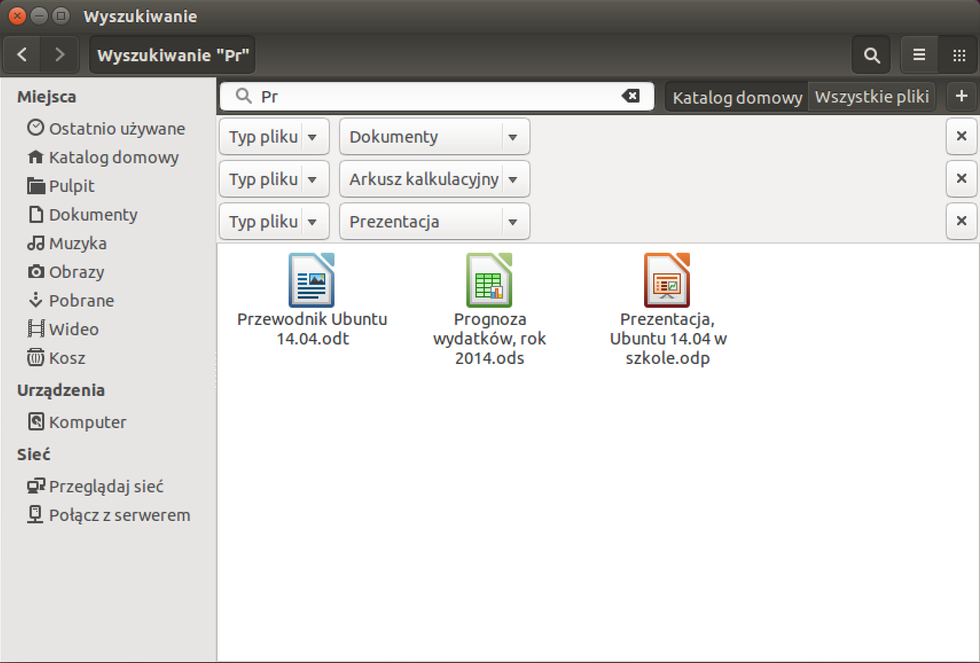
\includegraphics[width=\linewidth]{images/programy_nautilus2.png}
\end{center}

To, że Dash jest potężnym narzędziem i że pozwala wyszukiwać pliki, już wiemy. Ale pliki i katalogi możemy również wyszukiwać wykorzystując okno programu Pliki. Jak już wcześniej wspomnieliśmy, na pasku narzędzi okna programu znajduje się przycisk wyszukiwania (ikona szkła powiększającego). Po naciśnięciu przycisku wyszukiwania pojawi się pasek, w którym podajemy frazę (nazwę pliku lub katalogu) do wyszukania. Rezultaty wyszukiwania, podobnie jak w Dashu, możemy filtrować. Możemy określić, czy wyszukiwanie ma się odbywać w obrębie naszego katalogu domowego, czy w całym systemie. Możemy również podać dodatkowe kryteria wyszukiwania, określając jakiego typu plików szukamy.

\subsubsection{Używanie wielu okien lub wielu kart}
W przypadku kopiowania lub przenoszenia plików pomocne może być otwarcie wielu okien lub kart. Nowe okno programu Pliki można otworzyć na wiele sposób:
\begin{itemize}
\item wykorzystując panel menu i przycisk \menu{{Plik}>{Nowe okno}};
\item klikając prawym przyciskiem myszy ikonę programu Pliki na pasku Launchera i wybierając z menu kontekstowego \textcolor{ubuntu_orange}{Otwórz nowe okno};
\item wykorzystując skrót klawiaturowy \keys{CTRL + n}.
\end{itemize}
Program Pliki umożliwia również pracę z kartami, które także można otwierać na wiele sposobów:
\begin{itemize}
\item wykorzystując panel menu i przycisk \menu{Plik >{Nowa karta}};
\item klikając prawym przyciskiem myszy dowolny folder w oknie programu i wybierając z menu kontekstowego \textcolor{ubuntu_orange}{Otwórz w nowej karcie};
\item podwójne klikając środkowym przyciskiem myszy ikonę folderu, który ma zostać otwarty w nowej karcie;
\item wykorzystując skrót klawiaturowy \keys{CTRL + t}.
\end{itemize}
